\section{Experimental design, materials and methods}
\label{sec:methods}

\subsection{Collection}
\label{sec:collection}

The drives were recorded by the authors and by volunteers (see Acknowledgements) on public roads. The phones ran Sensor Logger \citep{sensorlogger} with the accelerometer, gyroscope, magnetometer, gravity, orientation and barometer sensors enabled, together with location and, where offered, the uncalibrated and compass streams. Every inertial channel was requested at a 10~ms interval. The barometer and location were left at the application's default, which \texttt{Metadata.csv} records as an interval of 0. The phones were \todo{state where and how the phones were held in the vehicle (mount, cradle, cup holder, loose), whether the mount changed during a drive, and which vehicles were used}. \todo{confirm that no additional hardware and no external reference receiver were used}. \Cref{tab:devices} lists the devices; \Cref{tab:channels} gives the rates the phones actually delivered, which fall short of the request on some devices (about 56~Hz for the Pixel 6a's inertial channels and about 60~Hz for the Samsung SM-S921U's gyroscope).

\subsection{Processing}
\label{sec:processing}

The raw recordings were converted to the processed trajectories by the \texttt{preprocess} command of the analysis package distributed with strapdown-rs \citep{strapdown-rs} (\texttt{analysis/src/analysis/preprocess.py}), run at 10~Hz. For each recording the steps are as follows.
\begin{enumerate}
\item Load the gyroscope, magnetometer, barometer, gravity, orientation and location files, and reject the recording if any is missing or the gyroscope covers less than 300~s. GNSS is taken from \texttt{LocationGps} when the recording has it and otherwise from \texttt{Location}.
\item Take specific force from \texttt{TotalAcceleration}. Where that file is absent (iOS), add \texttt{Gravity} to the linear acceleration in \texttt{Accelerometer}.
\item Outer-join all streams on their UTC timestamps, discard everything before the first GNSS fix, and average into 0.1~s bins. Because GNSS arrives at about 1~Hz, nearly every fix falls in a bin of its own, and bins without a fix keep empty GNSS columns.
\item Split the result wherever the inertial columns are empty for more than 5~s (the largest gap the strapdown-rs simulator accepts), trim incomplete rows from the ends, and drop any segment shorter than 300~s.
\item Download the three map tiles for the segment's bounding box, padded by a margin, through PyGMT \citep{wessel2019gmt}.
\end{enumerate}
Of the \numRawRecordings{} recordings, \numUsedRecordings{} yield processed trajectories. \texttt{segments.json} records the reasons for the other \numExcludedRecordings{}. One recording has no sensor data, one stops its inertial streams after 147~s, and \numNoBaroRecordings{} have no barometer. One recording was split at inertial dropouts into three kept trajectories (\texttt{2025-11-09\_17-34-01\_A}--\texttt{C}). In another, the two segments after a dropout were shorter than 300~s and were dropped, leaving \texttt{2025-06-11\_20-34-24\_A}.

Bin averaging is a boxcar decimation. It slightly shortens vector quantities whose direction changes within a bin; \Cref{sec:gravity} shows the effect on the gravity norm. Users who need the full rate or a different filter should start from the raw files.

\subsection{GNSS quality}
\label{sec:gnss}

\Cref{fig:gnss} shows the distribution of the accuracies the receivers reported. Across trajectories, the median reported horizontal accuracy is \numMedianHacc~m (trajectory medians range from \numHaccMin{} to \numHaccMax~m), the median vertical accuracy is \numMedianVacc~m, and the median speed accuracy is \numMedianSacc~m/s (\Cref{tab:trajectories}). Some devices report accuracy in a few discrete values, visible as steps in \Cref{fig:gnss}, so these figures are better read as the receiver's own coarse quality flag than as calibrated error statistics. The two platforms' location services also disagree on altitude. On \numAltIosCells{} road cells of \(0.002^\circ\) traversed above 15~m/s by both an iPhone and a Pixel 9 Pro, the iPhone altitude is lower by a median of \(\numAltIosMedian\)~m (interquartile range \(\numAltIosLow\) to \(\numAltIosHigh\)~m). The two other Android families agree with the Pixel 9 Pro to within \numAltAndroidMaxOffset~m. Altitude should therefore not be compared across platforms without care. Over the whole set, \numSentinelTotal{} fixes in \numSentinelTrajectories{} trajectories report a horizontal accuracy of 999~m or more, which marks a fix with no usable accuracy estimate.

\begin{figure}[t]
\centering
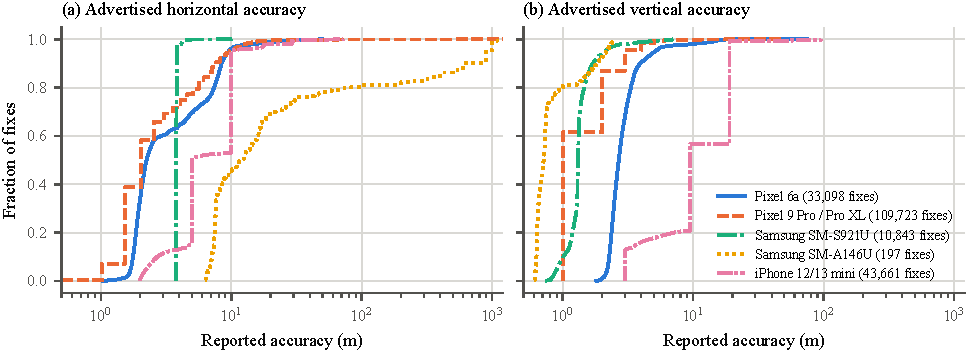
\includegraphics[width=\linewidth]{figures/fig_gnss_accuracy.pdf}
\caption{Empirical distribution of the horizontal (a) and vertical (b) accuracy reported with each GNSS fix in the processed trajectories, pooled by device family. Line styles distinguish families in addition to color.}
\label{fig:gnss}
\end{figure}

One trajectory is markedly worse than the rest. \texttt{2025-06-14\_21-17-02}, the only Samsung SM-A146U recording with data, delivered \numBadRawFixes{} location fixes in its raw file and \numBadFixes{} in the processed trajectory over \numBadSpan~s, a rate of \numBadFixRate{} fixes per second with gaps of up to \numBadMaxGap~s. Its median reported horizontal accuracy is \numBadHacc~m, and \numBadSentinels{} of its fixes report 999~m or more (up to \numBadHaccMax~m). It is kept in the release as a realistic poor-reception case. It dominates any aggregate that includes it, however (\Cref{sec:benchmark}), and users may prefer to report results with and without it.

\subsection{The operating-system gravity vector}
\label{sec:gravity}

The \texttt{Gravity} stream is not an accelerometer measurement. It is the operating system's fused estimate of the gravity direction, and its norm carries no information about local gravity. \Cref{fig:gravity} shows, for every raw sample, how far the norm falls below the largest norm in its recording. In \numGravRawPinnedRecordings{} of the \numUsedRecordings{} recordings that enter the processed set, every raw sample lies within 1~mGal (\(10^{-5}\)~m/s\(^2\)) of the recording's maximum. That maximum is a device constant: a median of \numGravPixel~m/s\(^2\) on the Pixel phones and \numGravSamsungApple~m/s\(^2\), standard gravity, on the Samsung SM-S921U and the iPhones. The exception, the Samsung SM-A146U, varies by tens of mGal below \numGravAfourteen~m/s\(^2\) (5th to 95th percentile of the deficit: \numGravAfourteenPfiveDeficit{} to \numGravAfourteenPninetyfiveDeficit~mGal). That variation is far larger than the gravity anomaly signal along these tracks. The 10~Hz bin averaging spreads the pinned norm slightly. In the processed files a median trajectory has \numGravTenHzPinnedMedian\% of its rows within 1~mGal of its maximum, which matches the figure reported by \citet{brodovsky2026dissertation}. Against the free-air anomaly map, the median per-trajectory signal-to-noise ratio of the resulting anomaly measurement is \numSnrGravity{} (best trajectory \numSnrGravityBest), below one on every trajectory \citep{brodovsky2026dissertation}. The \texttt{grav\_*} columns are useful as the operating system's attitude reference, not as a gravimeter.

\begin{figure}[t]
\centering
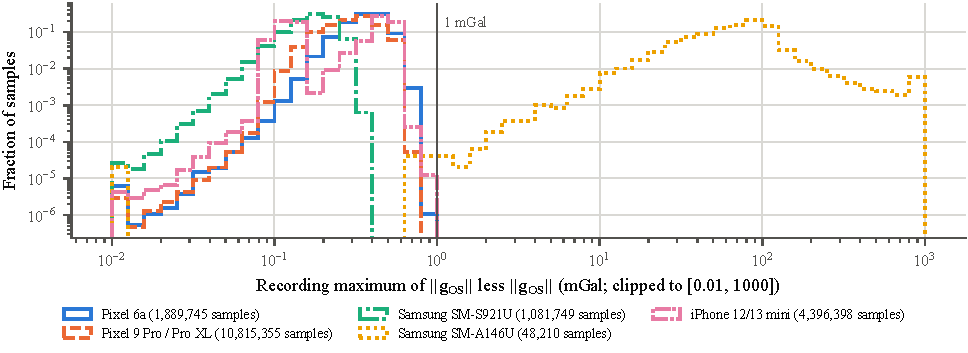
\includegraphics[width=\linewidth]{figures/fig_gravity_norm.pdf}
\caption{Norm of the operating-system gravity vector at the raw rate, expressed as its shortfall from the largest norm in the same recording and pooled by device family. Every family except the Samsung SM-A146U stays within 1~mGal (vertical line) of a fixed value throughout every recording.}
\label{fig:gravity}
\end{figure}

\subsection{The magnetometer}
\label{sec:magnetometer}

The \texttt{Magnetometer} stream is already hard-iron corrected by the operating system. In the \numHardIronCount{} processed recordings that also contain \texttt{MagnetometerUncalibrated}, the difference between the median uncalibrated and median calibrated field ranges from \numHardIronMin{} to \numHardIronMax~\(\mu\)T in magnitude. The calibrated field is still dominated by the vehicle. The median calibrated intensity of the processed trajectories ranges from \numMagIntensityMin{} to \numMagIntensityMax~\(\mu\)T, although all of them were recorded within a few hundred kilometres of each other and the geomagnetic field \citep{wmm} varies far less over that region. Fitting the heading-dependent pattern of the field leaves a body-fixed horizontal field of 56~\(\mu\)T at the median, larger than the Earth's horizontal field, and vehicle heading explains 57\% of the variance of the observed intensity \citep{brodovsky2026dissertation}. The median per-trajectory signal-to-noise ratio of the magnetic anomaly measurement against the WDMAM grid is \numSnrMagnetic{} (best \numSnrMagneticBest). The magnetometer direction can still support a heading measurement, but magnetic anomaly navigation from these phones would first need a vehicle calibration that the data do not provide.

\subsection{Replay, degradation and baselines}
\label{sec:benchmark}

Every processed trajectory can be replayed by the strapdown-rs simulator \citep{strapdown-rs}, which implements strapdown mechanization in the local-level frame after \citet{groves}. The recordings follow the east--north--up convention for specific force (\Cref{sec:processed}), so the simulator is run with \texttt{is\_enu = true}; it checks the declared frame against the data and refuses a mismatch. The simulator's GNSS degradation acts at two levels. A scheduler decides which recorded fixes the filter receives: all of them, one every fixed interval, or alternating on and off windows. A fault model then corrupts the delivered fixes, either with first-order autoregressive (AR(1)) noise on position and velocity together with inflated reported covariance \citep{wang2022noise}, with a slow drift, or with a step offset during a time window. Every random draw comes from a seeded generator, so a configuration file reproduces a run exactly.

The baselines in \Cref{tab:benchmark} use two scenarios. With \emph{full} GNSS, every recorded fix is delivered unmodified. With \emph{degraded} GNSS, one fix every 60~s is delivered. It carries AR(1) position error with a steady-state standard deviation of 35~m and a correlation time of 500~s, and AR(1) velocity error of 1.5~m/s with a correlation time of 100~s. The reported standard deviations are scaled by 5, so the measurement covariance grows by 25, and the seed is 42. Three filters were run: a loosely coupled extended Kalman filter (EKF), an unscented Kalman filter (UKF), and a Rao--Blackwellized particle filter (RBPF) after \citet{canciani2017airborne} \todo{confirm the particle count used for these runs; their configurations were not archived}. The simulator also passes the barometric relative altitude and a magnetometer-derived heading to the filters at its default schedule of one per second \todo{confirm which of these each filter consumed, and the strapdown-rs commit that produced the benchmark files}. No geophysical measurement was used. Performance is the horizontal great-circle distance between the filter's position and the recorded GNSS fix, evaluated at every recorded fix, including the fixes withheld from the filter. It is summarized per trajectory as a root-mean-square error (RMSE) and then across trajectories.

\begin{table}[t]
\centering
\caption{Reference baselines: horizontal RMSE against the recorded GNSS track, summarized over trajectories, and the median vertical RMSE. \(n\) is the number of trajectories on which the run completed. Errors of 10~km or more are given in kilometres.}
\label{tab:benchmark}
\small
\setlength{\tabcolsep}{4pt}
\begin{tabular}{llrrrrr}
\toprule
Filter & GNSS & \(n\) & Median (m) & Mean (m) & Max (m) & Vert.\ median (m) \\
\midrule
EKF & Full & 27 & 4.1 & 24.0 & 539.2 & 1.6 \\
 & Degraded & 27 & 440.4 & 611.4 & 2{,}436.1 & 23.4 \\
\midrule
UKF & Full & 27 & 4.0 & 24.0 & 542.8 & 1.6 \\
 & Degraded & 27 & 430.4 & 577.1 & 3{,}115.4 & 24.0 \\
\midrule
RBPF & Full & 27 & 1.9 & 181.7 & 3{,}628.5 & 1.6 \\
 & Degraded & 26 & 817.7~km & 941.9~km & 2{,}704.3~km & 445.7 \\
\bottomrule
\end{tabular}

\end{table}

With full GNSS, the EKF and UKF follow the recorded track to a median horizontal RMSE of \numEkfFullMedian{} and \numUkfFullMedian~m. On every trajectory except \texttt{2025-06-14\_21-17-02} the RMSE is at most \numEkfFullMaxOthers~m, while on that trajectory it is \numEkfFullBad~m (EKF) and \numUkfFullBad~m (UKF). This agreement mainly shows that the replay and the column conventions are consistent; it is not a measure of absolute accuracy (\Cref{sec:limitations}). With degraded GNSS, the median grows to \numEkfDegradedMedian~m (EKF) and \numUkfDegradedMedian~m (UKF). That is the regime in which an alternative aiding source has to prove itself, and the baseline that such a source should be compared against. The RBPF configuration that was used tracks well with full GNSS (median \numRbpfFullMedian~m), but it diverges in the degraded scenario: its median RMSE is \numRbpfDegradedMedian{} on the \numRbpfDegradedN{} trajectories that completed, and \numRbpfDegradedMissing{} did not complete. It is reported as a configuration that fails, not as a usable baseline. The scenario files and the per-trajectory results are included in the release (\Cref{sec:layout}).
